

\section{Detector Apparatus}
\label{sec:cmsexperiment:detector}



% overview
The CMS \cite{exhep:cms:Chatrchyan:2008aa} detector is a general-purpose apparatus operating at the LHC and is located about 100 meters underground at Point 5 of the LHC, close to the French village of Cessy, between Lake Geneva and the Jura mountains. As a general purpose detector, the CMS detector is designed to observe any new physics phenomena that the LHC might reveal \cite{cms:tdr2:Ball:2007zza}. At the designed LHC luminosity of \SI{e34}{\per\cm\squared \per\s}, on average about 20 inelastic collisions are superimposed on the event of interest every collision of bunch crossings, leading to a large flux of particles originating from the detector center to enter the detector every 25 ns. In order to discern them and trigger the interested events within 25 ns latency over the LHC run period until 2035, CMS detector is designed to be highly-segmented, radiation-hard and with good timing resolution \cite{exhep:cms:Chatrchyan:2008aa}.

\begin{figure}[ht]
    \centering
    \includegraphics[width=0.98\textwidth]{chapters/CMSExperiment/sectionDetector/figures/cmsDetector.png}
    \caption{The layout of the CMS detector \cite{cms:detectorOverview}.}
    \label{sec:cmsexperiment:detector:detectorOverview}
\end{figure}

% overview of structure
The apparatus layout of CMS detector is shown in Figure~\ref{sec:cmsexperiment:detector:detectorOverview} \cite{cms:detectorOverview}. The central feature of the CMS apparatus is a superconducting solenoid of 6 m internal diameter, providing a magnetic field of 3.8 T. Within the superconducting solenoid volume are a silicon pixel and strip tracker, a lead tungstate crystal electromagnetic calorimeter, and a brass and scintillator hadron calorimeter, each composed of a barrel and two endcap sections. Muons are measured in gas-ionization detectors embedded in the steel flux-return yoke outside the solenoid. Additional forward calorimetry complements the coverage provided by the barrel and endcap detectors. The more details of these sub-systems, including magnet,  are discussed in this section. 

% To achieve the physics goal in the LHC environment, the design of each CMS sub-detectors are driven by the following performance requirement.

% \begin{itemize}
%     \item Magnets and Muon chamber: Good muon identification, energy resolution, charge determination.
%     \item Pixel and Tracker: Good charge hadron track reconstruction efficiency. Good displaced vertex tagging for $b$, $\tau$ identification.
%     \item ECAL: Good electromagnetic energy resolution. $\pi^0$ rejection. Efficient photon and lepton isolation at high luminosities.
%     \item HCAL: Good missing-transverse-energy and dijet-mass resolution
% \end{itemize}



\subsection{Magnet}
% overview
The CMS superconducting magnet \cite{cms:magnetTdr:Acquistapace:1997fm} is used to provide bending to the charged particles as they traverse, which is crucial to both particle identification and momentum measurement. The internal magnetic filed is 4 Tesla with 2.6 GJ stored energy and is generated by a superconducting solenoid surrounded by a set of return york. The solenoid is 12.5 m in length, 6.3 m in diameter and 200 ton in weight, consist of 41.7 MA-turn of wire. The radiation thickness of the solenoid is 4.9 $\chi_0$, which further prevents hadrons from entering the muon system. The solenoid is surrounded and mechanically supported by the iron return yokes, which direct the outer magnetic in the muon system. The yoke, consist of 5 barrel wheels and two endcaps, has an outer diameter of 14 m and a total weight of 10000 tons. Both barrel and endcap return yoke have three iron layers with thickness of 300/630/630 mm and 250/600/600 mm, respectively.



\subsection{Inner Tracking System}
% overview
The inner tracking system \cite{cms:trackerTdr:CMS:1997tlf} is used to measure the trajectories of charged particles. Covering region with $|\eta|<2.5$, it is consist of two major parts: pixel detector and Silicon strip tracker, layout of which is shown in Figure~\ref{sec:cmsexperiment:detector:trigger}. 


\begin{figure}[ht]
    \centering
    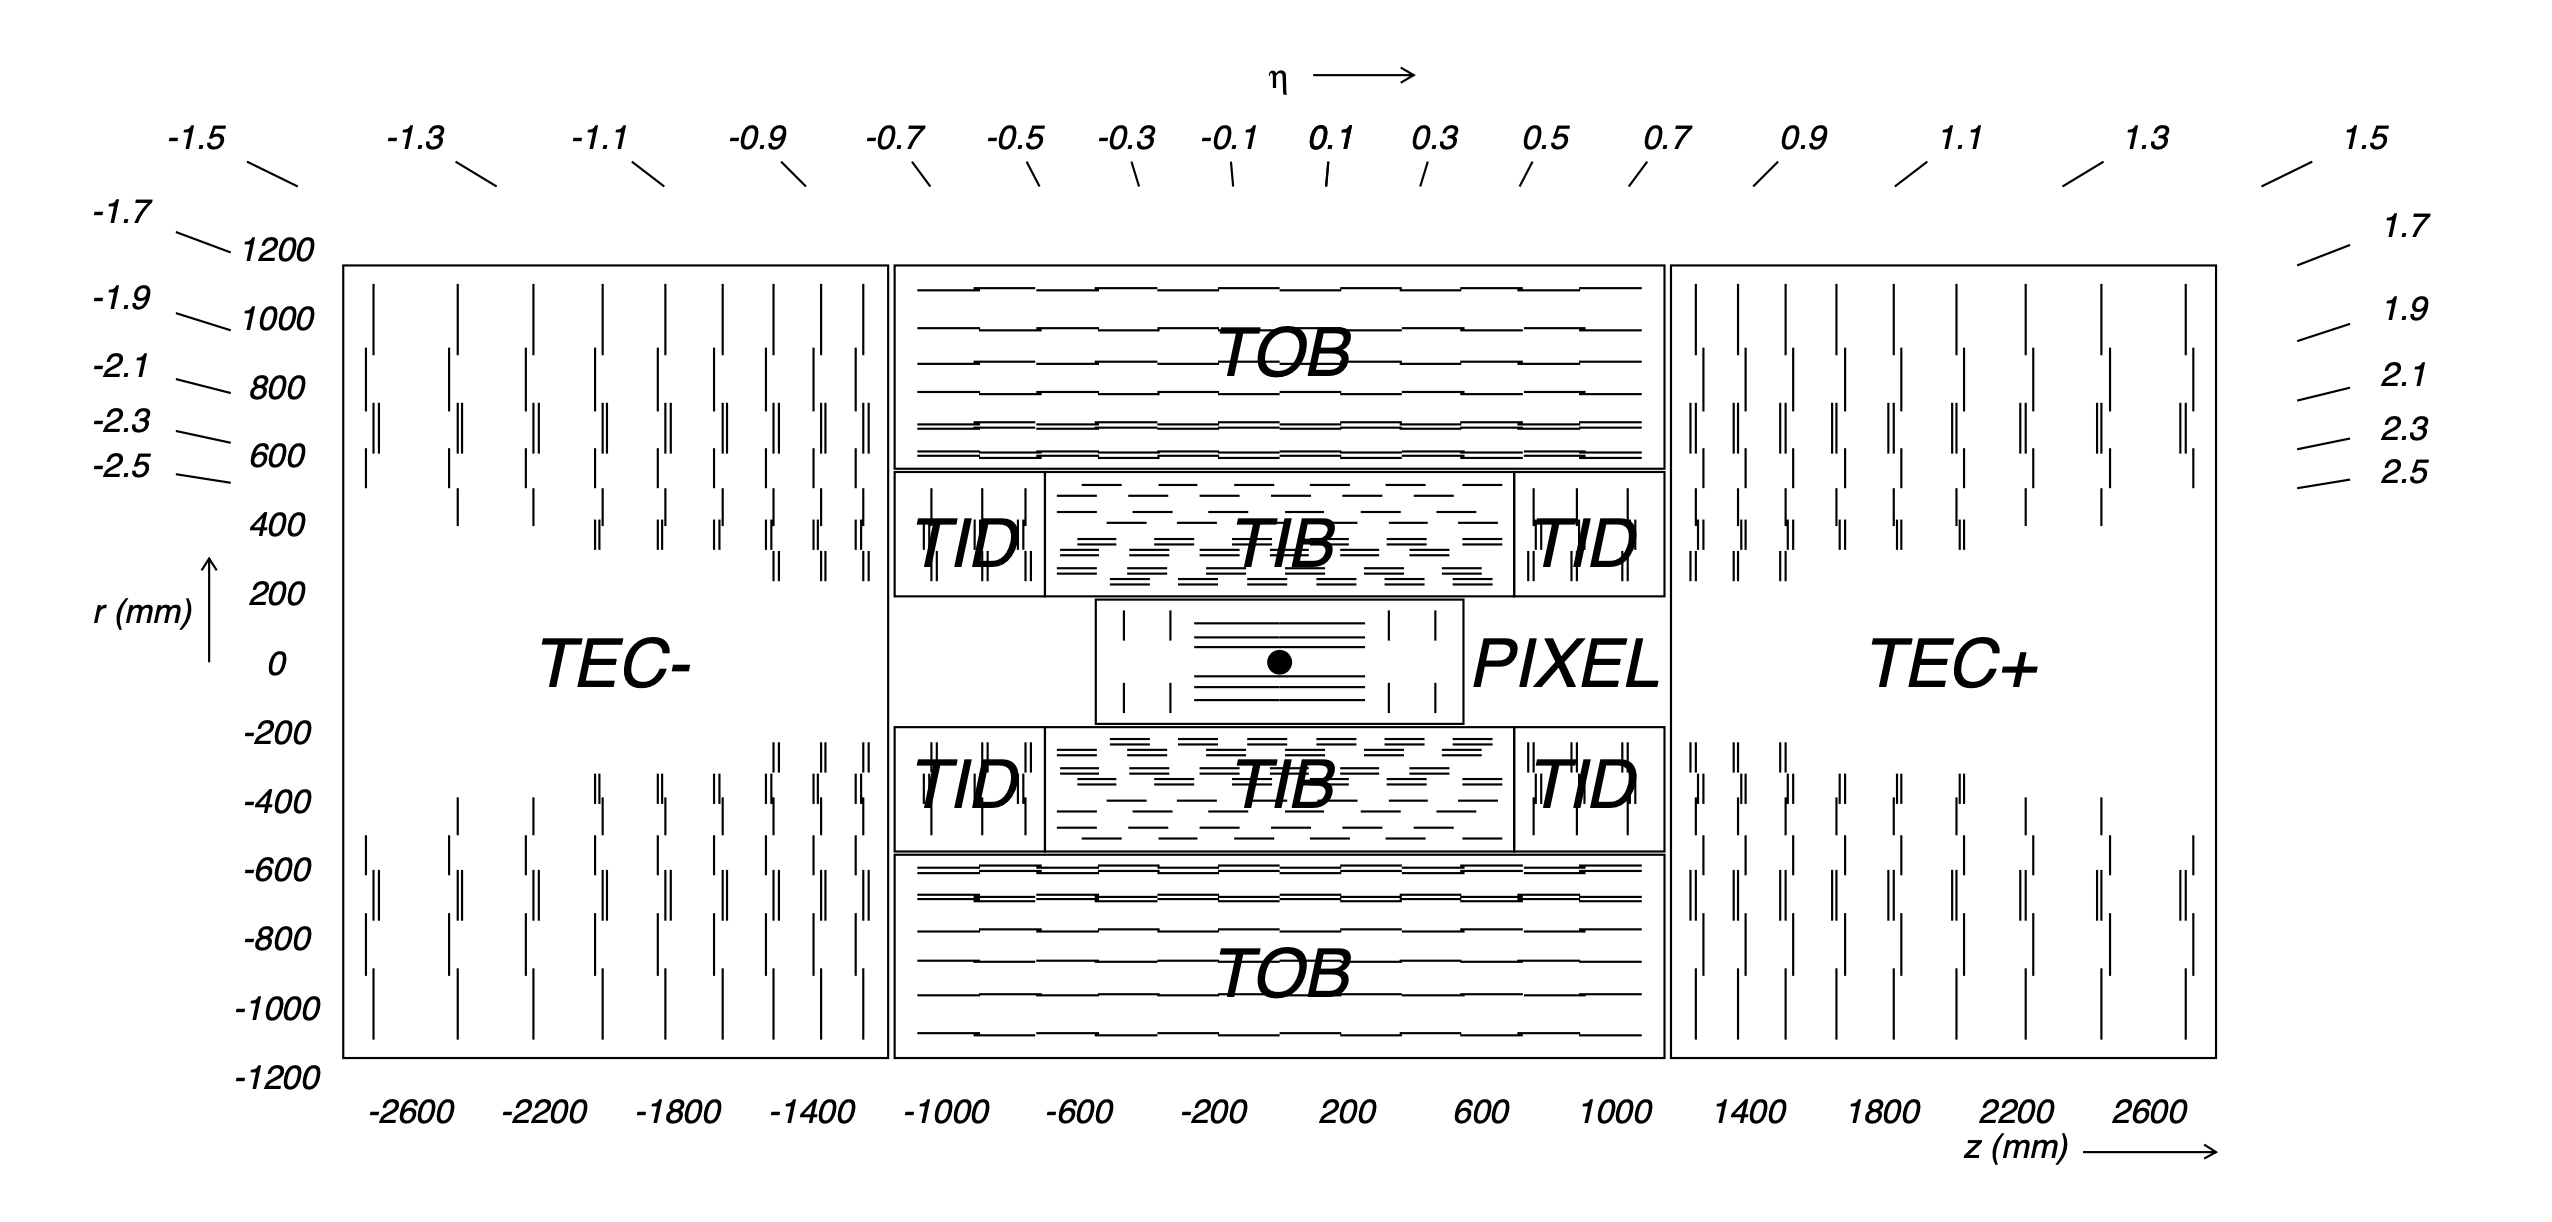
\includegraphics[width=0.98\textwidth]{chapters/CMSExperiment/sectionDetector/figures/tracker.png}
    \caption{The layout of the CMS inner tracking system \cite{exhep:cms:Chatrchyan:2008aa}. It is consist of pixel detector and silicon strip tracker (TIB/TID, TOB, TEC), covering regions with $|\eta|<2.5$. }
    \label{sec:cmsexperiment:detector:tracker}
\end{figure}


\begin{figure}[ht]
    \centering
    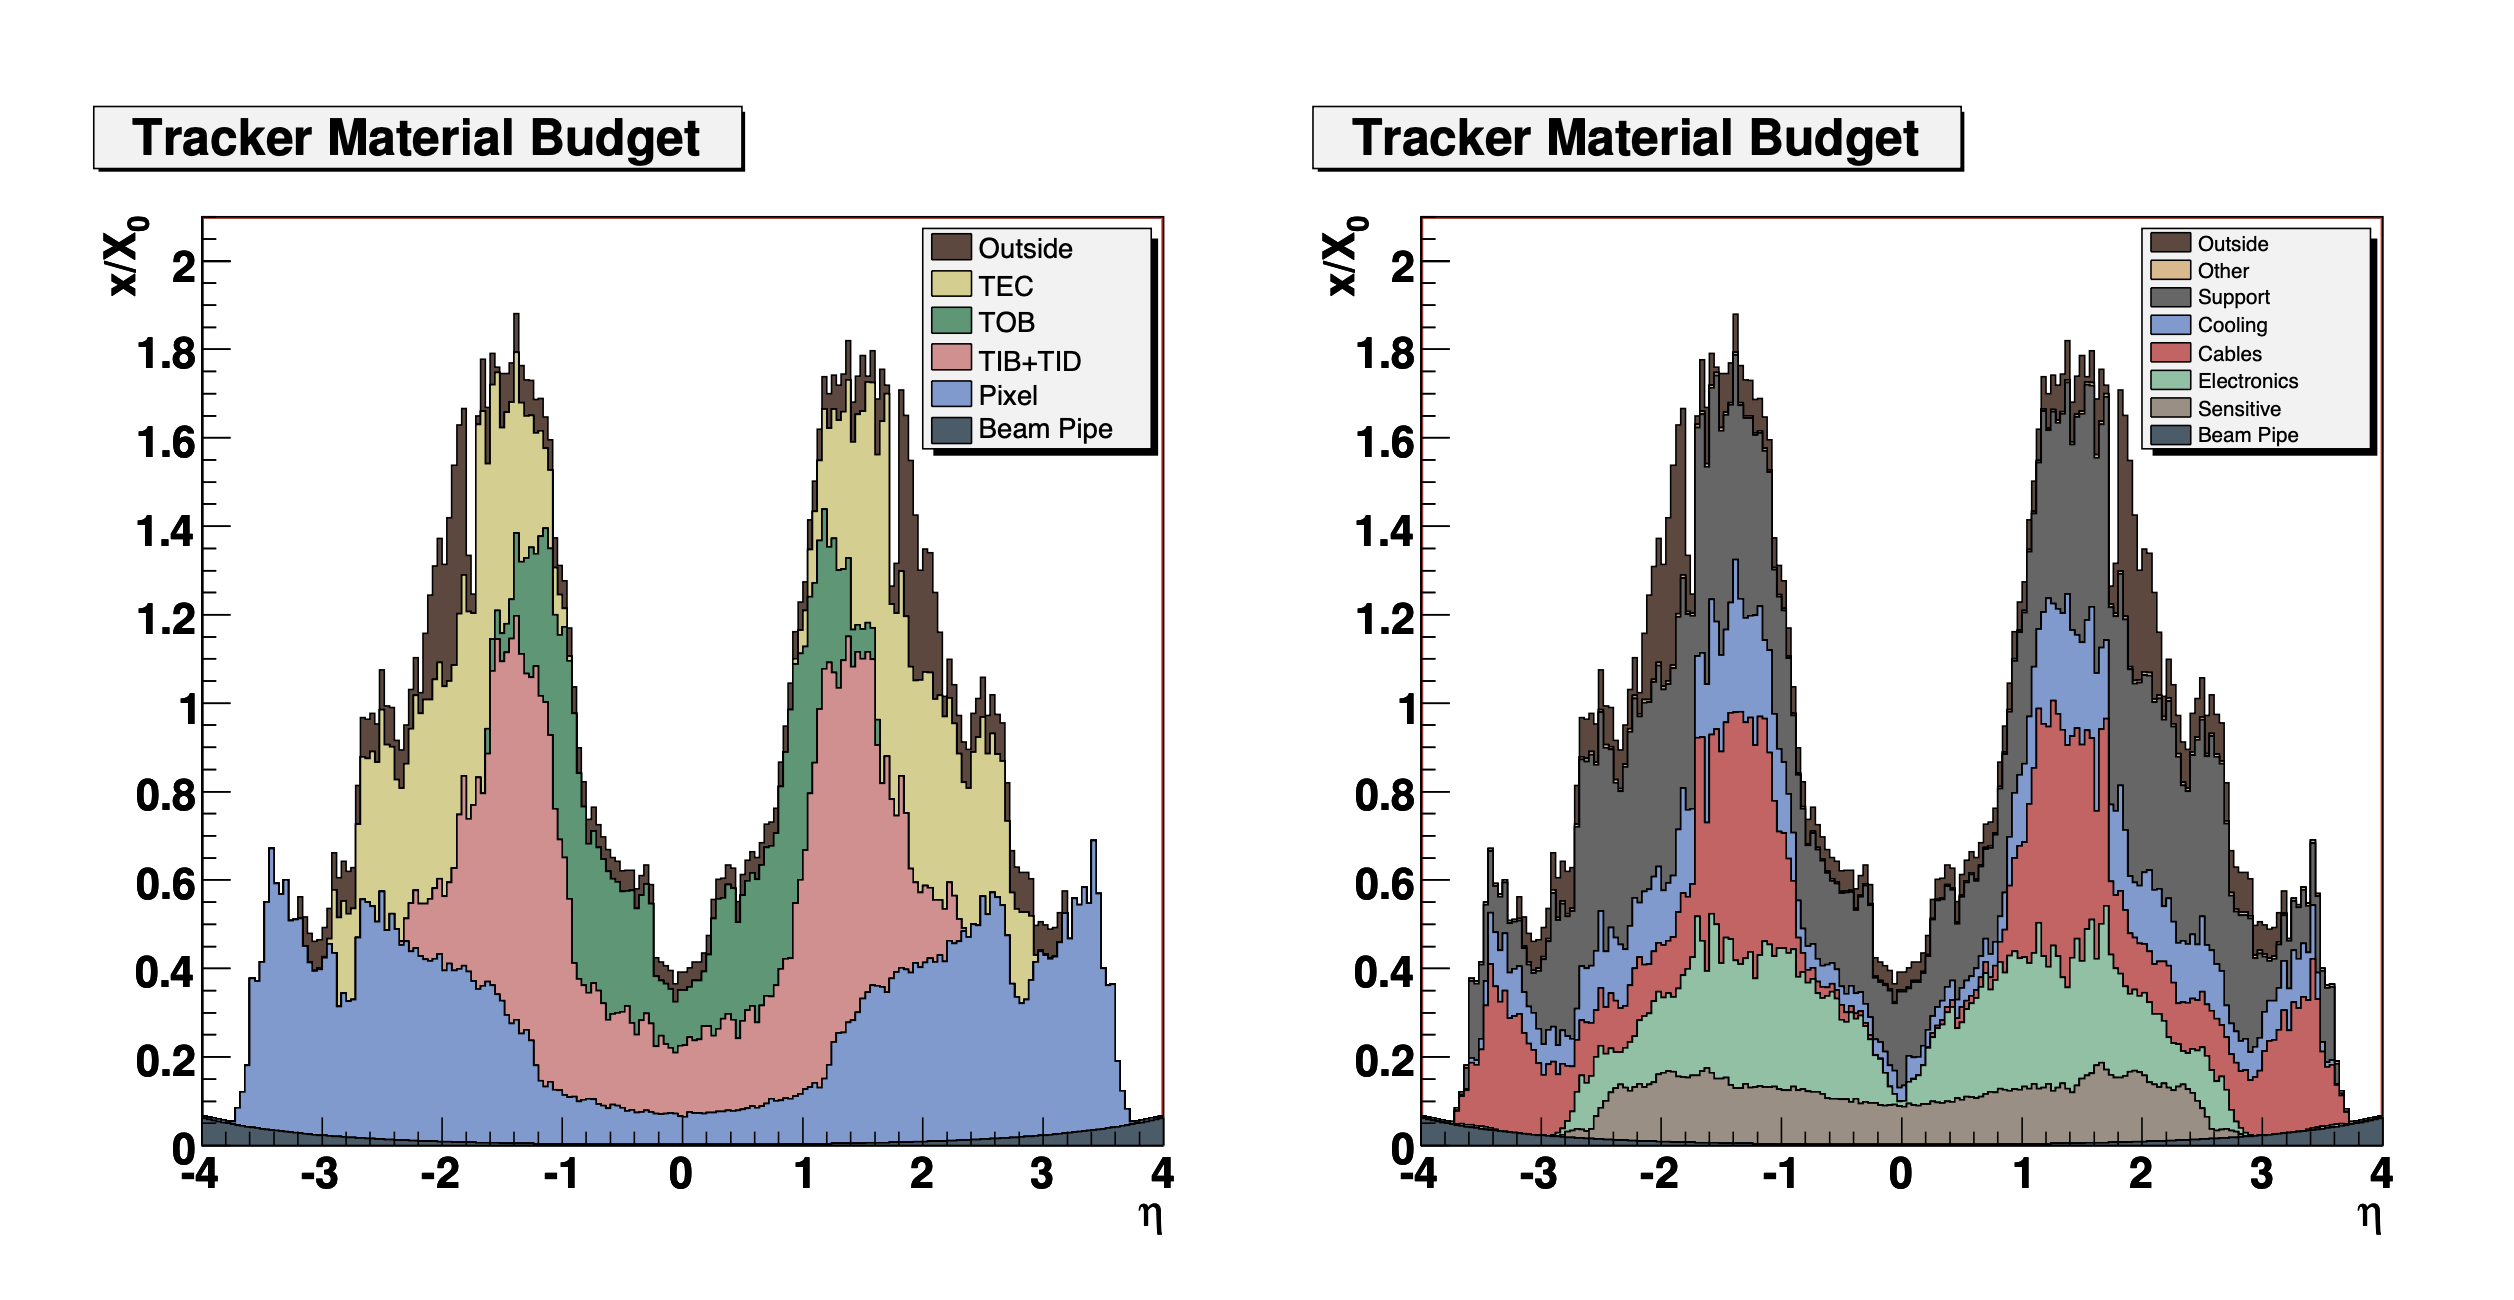
\includegraphics[width=0.98\textwidth]{chapters/CMSExperiment/sectionDetector/figures/trackerMaterial.png}
    \caption{The material thickness of inner tracking system before ECAL.}
    \label{sec:cmsexperiment:detector:trackerMaterial}
\end{figure}


% pixel
The pixel detector, shown in the center of Figure~\ref{sec:cmsexperiment:detector:trigger}, is consist of three cylindrical layers of pixel detector modules at radii of 4.4, 7.3, and 10.2 cm, totaling 66 million pixels with area of 1 \si{\m \squared}. It is capable of producing three high precision 3D spacial hits for each charged particle. 

% tracker
 The silicon strip tracker system is right outside the pixel detector in the region of $20<r<116$ cm and $|z|<282$ cm. The tracker system has three parts: \acrfull{tibtid}, \acrfull{tob} and \acrfull{tec}, with a total of 9.3 million channels and 198 \si{\m \squared} active silicon area. The silicon strip modules in the barrel are lied out in cylindrical shapes with their strips parallel to the Z direction to measure $r-\phi$ coordinates. In comparison, those in the endcap region are in the shape of disks and place their strips in radial direction to measure the $Z-\phi$ coordinates. In addition to measuring the 2D coordinates, the first two cylinders of TIB and TOB, the first two disks of TID and TEC, as well as the fifth ring of TEC, are double-sided by placing a second micro-strip detector module back-to-back to the first module with a stereo angle of 100 mrad. This small stereo angle allows the measurement of the third spacial coordinates: $Z$ in the barrel (TIB and TOB) and $r$ on the endcap (TID and TEC). Such tracker design ensures to acquire at least 9 hits in the silicon strip tracker with at least 4 of them being stereo measurements. 

% Figure 3.3 shows the material budget of the CMS tracker in units of radiation length. It increases from 0.4 $\chi_0$ at $|\eta| =0$ to about 1.8 $\chi_0$ at $|\eta| =1.4$, beyond which it falls to about 1 $\chi_0$ at $|\eta| =2.5$.



\begin{figure}[ht]
    \centering
    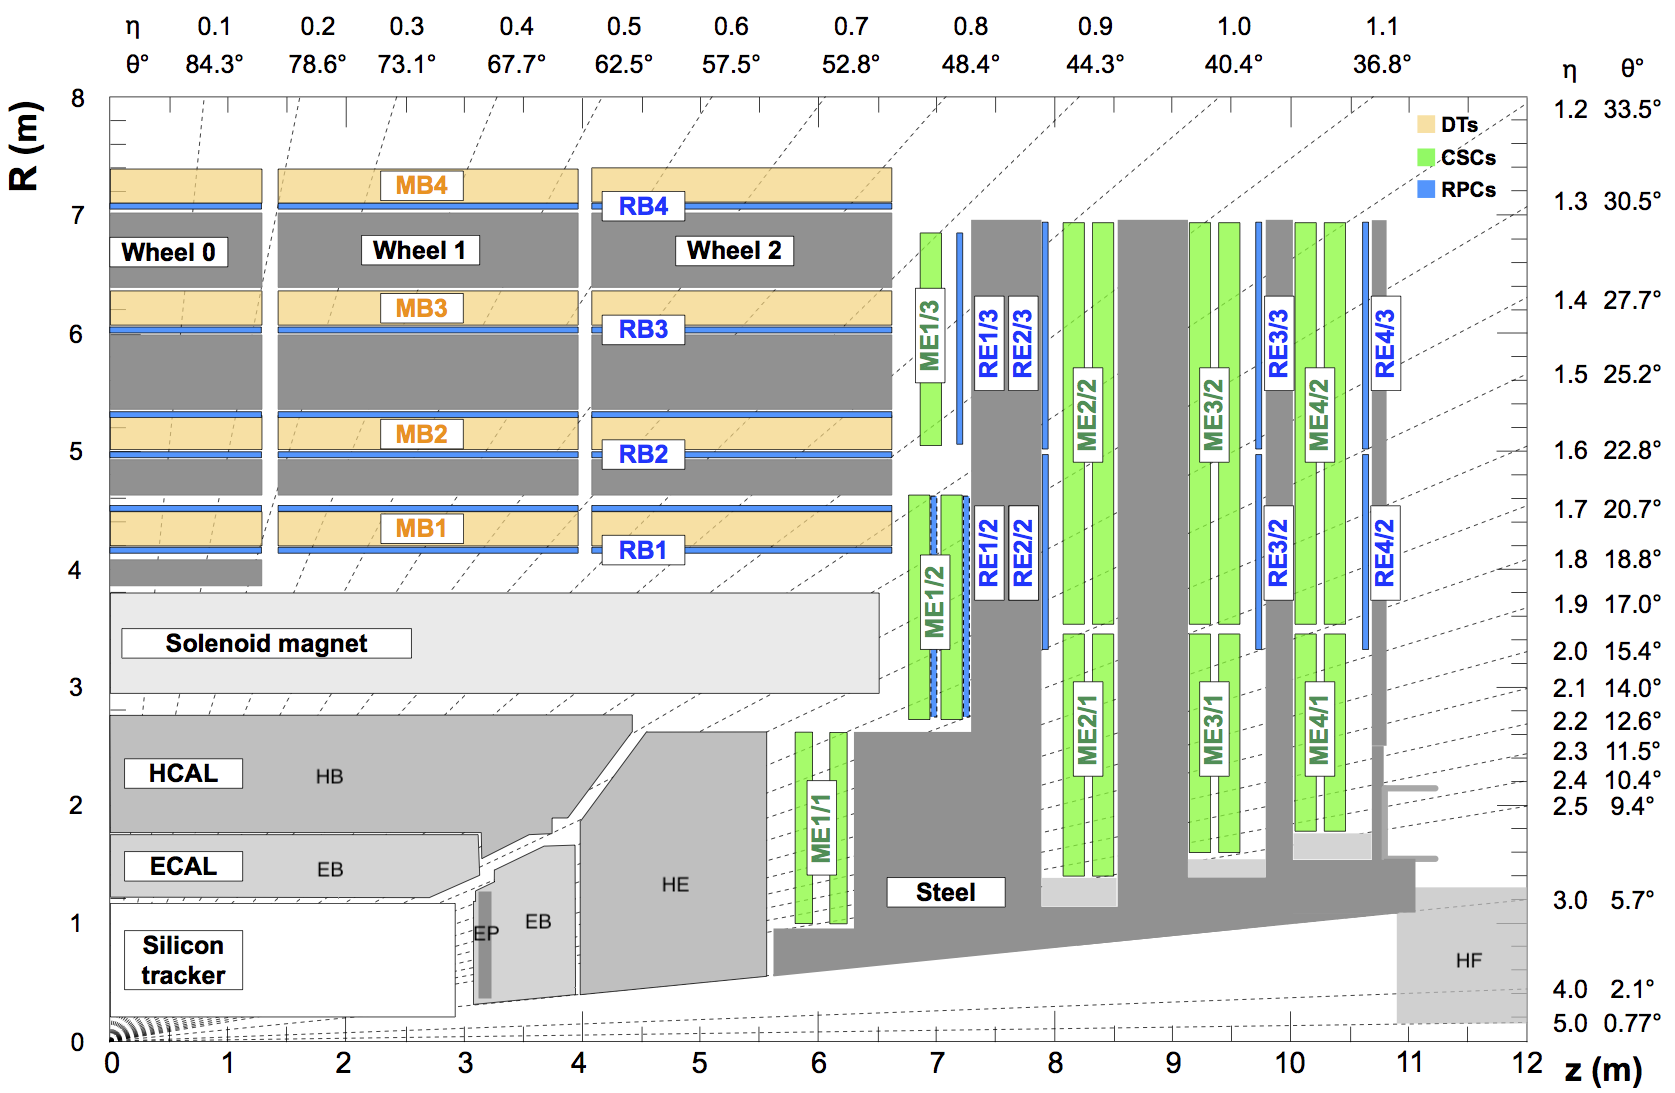
\includegraphics[width=0.98\textwidth]{chapters/CMSExperiment/sectionDetector/figures/detectorLayout.png}
    \caption{The layout of the CMS tracker, ECAL, HCAL, Magnets and muon system on the Z-r plane \cite{cms:muonChamberWebsite}. The full coverage of pseudorapidity is up to $\eta=5$. The details of tracker is shown in Figure~\ref{sec:cmsexperiment:detector:tracker}. }
    \label{sec:cmsexperiment:detector:detectorLayout}
\end{figure}




\subsection{Electromagnetic Calorimeter (ECAL)}
%  overview
The CMS electromagnetic calorimeter (ECAL) \cite{cms:ecalTdr:CMS:1997ysd} is used to measure the energy of electromagnetic showers. As shown in Figure~\ref{sec:cmsexperiment:detector:detectorLayout}, ECAL is located right outside the tracking system discussed in the Section~\ref{sec:exp:trigger}. ECAL consists of the barrel part (EB), the endcap part (EE) and a preshower system (EP) in front of EE. EB and EE are hermetic homogeneous calorimeter made of lead tungstate crystals with \acrfull{apd} and \acrfull{vpt} as readout sensors respective, while the PS is a sampling calorimeter with lead-silicon alternating layers to enhance the spatial resolution in the EE region. The total ECAL material thickness is larger than 25 $\chi_0$ and about 1.1 $\lambda_I$.

% EB
The barrel part of the ECAL (EB) covers the pseudorapidity range of $|\eta|< 1.479$ and consists of 61200 crystals arranged in a 170x360 $\eta - \phi$ grid, with 8.14 $m^3$ of total crystal volume and 67.4 tons of weight. The crystals have a tapered shape mounted in a quasi-projective distribution, in which the crystal axis has 3\degree angle with respect to the vector from the origin to minimize chances of cracks aligned with the particle trajectories. The crystal cross-section corresponds to approximately $0.0174 \times 0.0174$ in $\eta - \phi$ or $22 \times 22$ $mm^2$ at the front face of crystal, and $26\times26$ $mm^2$ at the rear face. The crystal length is 230 mm corresponding to 25.8 $\chi_0$.

% EE
The endcaps (EE) cover the rapidity range $1.479 < |\eta| < 3.0$ and is consist of 7324 identically shaped crystals grouped in mechanical units of 5x5 crystals (supercrystals, or SCs), with 2.90 $m^3$ of total crystal volume and 24.0 tons of weight. The crystals are arranged in a rectangular x-y grid, with the crystals pointing at a focus 1300 mm beyond the interaction point, giving off-pointing angles ranging from 2 to 8 degrees. The crystals have a front face cross section $28.62\times28.62$ $mm^2$, a rear face cross section $30\times30$ $mm^2$ and a length of 220 mm corresponding to 24.7 $\chi_0$.

% preshower
A preshower detector (EP) is placed in front of EE in $1.479 < |\eta| < 2.6$ to increase the space resolution of electromagnetic showers and better identify neutral pions $\pi^0 \to \gamma \gamma$ in the endcap. EP is a sampling calorimeter with two lead-silicon layers. On each layer, the lead radiators initiate electromagnetic showers from incoming photons and electrons, while silicon strip sensors placed after each radiator measure the deposited energy and the transverse shower profiles. The directions of silicon strips on the two layers are orthogonal to each other. The material thickness of the first and second layer are 2 $\chi_0$ and 1 $\chi_0$ respective, with a total mechanical thickness of 20 cm.



\subsection{Hadron Calorimeter (HCAL)}
% overview
The CMS Hadron Calorimeter \cite{cms:hcalTdrCMS:1997xji} is used to measure the energy of hadrons and determine the missing transverse energy. HCAL consists of four parts: the HCAL in barrel region (HB) between ECAL and magnets, HCAL in the endcap region (HE), the forward hadronic calorimenter (HF) and a small section outside the magnetic (HO) in the barrel region to catch rare hadronic punch through before muon system. As shown in Figure~\ref{sec:cmsexperiment:detector:detectorLayout}, HB and HE are designed right outside the ECAL; FH is in the high pseudorapidity region outside the whole CMS endcap.

% HB, HE, HO
HB and HE are a sampling calorimeter covering $|\eta|< 1.3$, $1.3<|\eta|< 3.0$ respectively. They use brass absorber ($70\%$ Cu and $30\%$ Zn) and plastic scintillators for readout. HO covers the same $|\eta|< 1.3$ range as HB but uses iron as absorber enhance the material thickness in HB especially in the low $\eta$ region. With HO, the total material thickness of the HCAL is about 11.8 $\lambda_I$ make sure the hadronic leakage to muon is very rare. Totally, HCAL has about 7000 scintillators channels, granularity of which is $\Delta \eta \times \Delta \phi = 0.087 \times 0.087$ in the HB, OB and $1.3<|\eta|< 1.6$ part of HE and $\Delta \eta \times \Delta \phi = 0.017 \times 0.017$ in the rest part of HE.

% HF
HF is a sampling calorimeter covering $3.0 < |\eta| < 5$. It is essentially a cylindrical steel structure with an outer radius of 130.0 cm and with fibers piecing from the back in Z direction at two different depths. The front face of the calorimeter is located at 11.2 m from the interaction point. The absorber are made of steel installed perpendicular to beam pipe with a total material depth of 10 $\lambda_I$. The active material is quartz fibres (fused-silica core and polymer hard-cladding) installed in parallel with the beam pipe. When particle showers in the HF, a small part of Cherenkov light generated at the surface of quartz fibres is captured. To distinguish the electromagnetic shower vs hadronic shower, two different the penetration depth of fibers are used, long fiber span the entire HF, while short fibers start from 22 cm behind the HF front surface and extend to the back. These fibers are bundled to form $\Delta \phi \times \Delta \eta = 0.175 \times 0.175$ towers. 


\subsection{Muon System}
% overview
The CMS muon system \cite{cms:muonChamberTdr:CMS:1997iti} is designed outside the solenoid hosted in the return yoke to measure the tracks of muons. The system consists of barrel detector (MB) covering $|\eta|<1.2$ and endcap detectors (ME) covering $0.9 < |\eta| < 2.4$. 

% MB RPC
The barrel detector has 250 chambers in total which hosts 250 \acrfull{dt} and 480 \acrfull{rpc}. The chambers are  arranged in 4 concentric stations in the yoke, each of which is in turn divided into 5 wheels with 12 sectors on each wheel. The two inner most stations, labeled as MB1 and MB2 in Figure~\ref{sec:cmsexperiment:detector:detectorLayout}, has two RPCs sandwiching a DT, while The 2 outermost stations, MB3 and MB4 in Figure~\ref{sec:cmsexperiment:detector:detectorLayout}, consist of packages of a DT coupled to a layer on the inner side made of 1, 2, or 4 RPCs, depending on the sector and station.
Each DT in MB1, MB2 and MB3 has 12 layers of drift tubes divided into 3 groups of 4 consecutive layers or 3 superlayers. Two with wire parallel to Z direction measure $r-\phi$ coordinates, the middle one with wire perpendicular to Z direction measures $r-z$ coordinates. DTs in MB4 only have two superlayers for measurement of $r-\phi$ coordinates. RPCs are attached to DTs to improve the responding time necessary for triggers. Each RPC detector has a bakelite chamber with two 2 mm wide gaps and operates in avalanche mode biased by a high voltage. 

% ME
The endcap detector has 469 \acrfull{csc}s and 432 RPCs on two sides in the yokes that close the solenoid. The ME consists of 4 stations ME1-ME4. The disk of ME1 is divided into 3 concentric rings, while two rings for ME2-ME4. The details of the layout of CSCs and RPCs in ME are shown in Figure~\ref{sec:cmsexperiment:detector:detectorLayout}. Each CSC is trapezoidal in shape and consists of 6 gas gaps, each gap having a plane of radial cathode strips and a plane of anode wires running almost perpendicularly to the strips and measuring hits with 3D coordinates.

